\documentclass{beamer}

\usepackage{amsmath}
\usepackage{pgfplots}
\usepgfplotslibrary{fillbetween}
\usepackage{minted}
\usepackage[T1]{fontenc}
\usepackage{multicol}

\author{Tom Deakin}
\title{OpenMP for Computational Scientists}
\subtitle{The Pi program}

\begin{document}

\frame{\titlepage}

%-------------------------------------------------------------------------------

\section{Outline}
\begin{frame}
\frametitle{Outline}
\begin{itemize}
  \item Data sharing clauses
  \item The Pi program
  \item Critical regions
  \item Atomics
  \item False sharing issues
  \item Reductions
\end{itemize}
\end{frame}
%-------------------------------------------------------------------------------

\section{Calculating Pi}
\begin{frame}
\frametitle{Integration to calculate Pi}
$$\int_{0}^{1} \frac{4}{1+x^2} dx = \pi$$

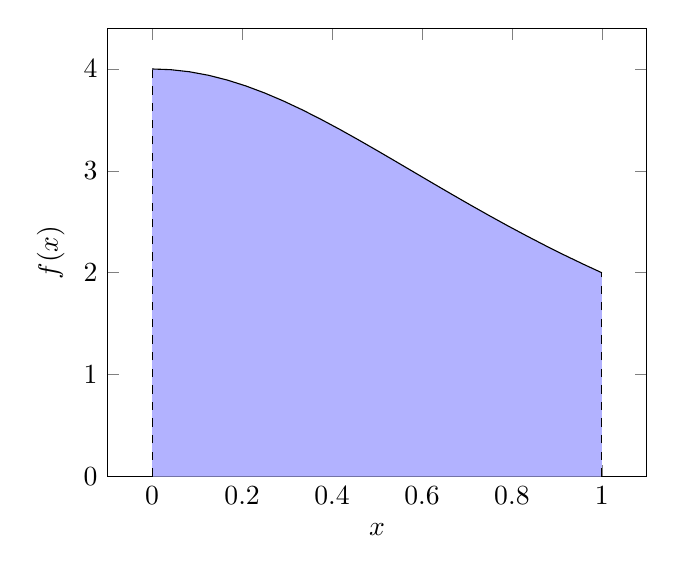
\begin{tikzpicture}
  \begin{axis}[xlabel={$x$},ylabel={$f(x)$},ymin=0]
    \addplot [name path=A, domain=0:1] {4/(1+x*x)};
    \addplot[dashed] coordinates {(0,0) (0,4)};
    \addplot[dashed] coordinates {(1,0) (1,2)};
    \path [name path=axis] (axis cs:0,0) -- (axis cs:1,0);
    \addplot[blue!30] fill between [of=A and axis, domain=0:1];
  \end{axis}
\end{tikzpicture}
\end{frame}

%-------------------------------------------------------------------------------
\begin{frame}
\frametitle{Trapezoidal rule}
Sum the area of the boxes. Choose a small \emph{step} size to generate lots of boxes, and increase accuracy.
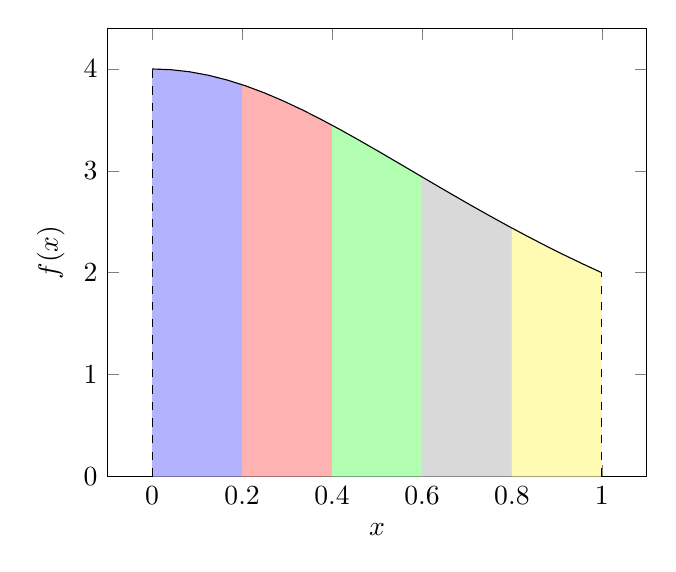
\begin{tikzpicture}
  \begin{axis}[xlabel={$x$},ylabel={$f(x)$},ymin=0]
    \addplot [name path=A, domain=0:1] {4/(1+x*x)};
    \addplot[dashed] coordinates {(0,0) (0,4)};
    \addplot[dashed] coordinates {(1,0) (1,2)};
    \path [name path=axis] (axis cs:0,0) -- (axis cs:1,0);
    \addplot[blue!30] fill between [of=A and axis, soft clip={domain=0:0.2}];
    \addplot[red!30] fill between [of=A and axis, soft clip={domain=0.2:0.4}];
    \addplot[green!30] fill between [of=A and axis, soft clip={domain=0.4:0.6}];
    \addplot[gray!30] fill between [of=A and axis, soft clip={domain=0.6:0.8}];
    \addplot[yellow!30] fill between [of=A and axis, soft clip={domain=0.8:1}];
  \end{axis}
\end{tikzpicture}
\end{frame}

%-------------------------------------------------------------------------------
\begin{frame}[fragile]
\frametitle{Code}
\begin{minted}[linenos,breaklines]{fortran}
  step = 1.0/num_steps
  do ii = 1, num_steps
    x = (ii-0.5)*step
    sum = sum + (4.0/(1.0+x*x))
  end do
  pi = step * sum
\end{minted}
With 100,000,000 steps, this takes 0.368s on my laptop.
\end{frame}

%-------------------------------------------------------------------------------
\subsection{Critical regions}
\begin{frame}[fragile]
\frametitle{Parallelising with critical}
Add simple \mintinline{fortran}|!$omp parallel do|, but need to be careful changing the \mintinline{fortran}|sum| as this will be \emph{shared} between threads.

A \mintinline{fortran}|critical| region only allows one thread to excute at any one time. No guarentees of ordering.

\begin{minted}[linenos,breaklines]{fortran}
  step = 1.0/num_steps
  !$omp parallel do private(x)
  do ii = 1, num_steps
    x = (ii-0.5)*step
    !$omp critical
    sum = sum + (4.0/(1.0+x*x))
    !$omp end critical
  end do
  !$omp end parallel do
  pi = step * sum
\end{minted}

This takes 426.1s on my laptop (4 threads)!
\end{frame}

%-------------------------------------------------------------------------------
\subsection{Atomics}
\begin{frame}[fragile]
\frametitle{Atomics}
A \mintinline{fortran}|critical| region protects a whole block of code. For a single operation, can use \mintinline{fortran}|atomic| instead.

Atomic operations are with respect to the memory access of a scalar variable {\tt x}.

\begin{itemize}
  \item \mintinline{fortran}|read| for \mintinline{fortran}|v = x|
  \item \mintinline{fortran}|write| for \mintinline{fortran}|x = expr|
  \item \mintinline{fortran}|update| for \mintinline{fortran}|x = x op expr|
  \item \mintinline{fortran}|capture| for read and write/update. The result is retained: \mintinline{fortran}|x = x op expr; v = x|
\end{itemize}

Not specifying an atomic clause defaults to \mintinline{fortran}|update|.
\end{frame}

%-------------------------------------------------------------------------------
\begin{frame}[fragile]
\frametitle{Atomic pi}
\begin{minted}[linenos,breaklines]{fortran}
  step = 1.0/num_steps
  !$omp parallel do private(x)
  do ii = 1, num_steps
    x = (ii-0.5)*step
    !$omp atomic
    sum = sum + (4.0/(1.0+x*x))
  end do
  !$omp end parallel do
  pi = step * sum
\end{minted}
This takes 8.3s on my laptop (4 threads).
\end{frame}

%-------------------------------------------------------------------------------
\subsection{Avoiding critical regions}
\begin{frame}
\frametitle{Independent summation}
Both methods cause threads to synchronise for every update to \mintinline{fortran}|sum|.
But each thread could compute a partial sum independently, synchronising once to total at the end.

Make \mintinline{fortran}|sum| an array of length equal to the number of threads.
Each thread stores its partial sum, and the array is totally by the master thread serially at the end.
As it's \emph{shared memory}, the \mintinline{fortran}|sum| array can be read just fine on the master rank.
\end{frame}

%-------------------------------------------------------------------------------
\begin{frame}[fragile]
\frametitle{Independent summation}
\begin{minted}[linenos,breaklines]{fortran}
  step = 1.0/num_steps
  !$omp parallel private(x,tid)
  tid = omp_get_thread_num()
  sum(tid+1) = 0.0
  !$omp do
  do ii = 1, num_steps
    x = (ii-0.5)*step
    sum(tid+1) = sum(tid+1) + (4.0/(1.0+x*x))
    !$omp flush(sum)
  end do
  !$omp end do
  !$omp end parallel
  do ii = 1, nthreads
    pi = pi + sum(ii)
  end do
  pi = pi * step
\end{minted}
This takes 2.8s on my laptop (4 threads).
\end{frame}

%-------------------------------------------------------------------------------
\section{False sharing}
\begin{frame}
\frametitle{False sharing}
This code is susceptible to \emph{false sharing}.
This occurs when threads update data on the same cache line.
This triggers that the cache line is synchronised across all cores, and reread before being updated by the tread.
This is an example of \emph{cache thrashing}.
The performance is reduced as threads must wait for the cache lines to refresh.
\end{frame}

%-------------------------------------------------------------------------------
\begin{frame}[fragile]
\frametitle{First private pi}
Can use data sharing clauses to our advantage here. Give each thread a scalar copy of \mintinline{fortran}|sum| to compute their partial sum, and reduce with only one critical (or atomic) region at the end.
No false sharing, as value is just a single number (i.e.\ a register).
\begin{minted}[linenos,breaklines]{fortran}
  step = 1.0/num_steps
  !$omp parallel private(x) firstprivate(sum)
  !$omp do
  do ii = 1, num_steps
    x = (ii-0.5)*step
    sum = sum + (4.0/(1.0+x*x))
  end do
  !$omp end do
  pi = pi + sum
  !$omp end parallel
  !$omp critical
  pi = pi * step
  !$omp end critical
\end{minted}
This takes 0.104s on my laptop (4 threads).
\end{frame}

%-------------------------------------------------------------------------------
\section{Reductions}
\begin{frame}[fragile]
\frametitle{Reductions}
Much simpler to use the OpenMP \mintinline{fortran}|reduction| clause on a worksharing loop.
Specify the operation and the variable.
\begin{multicols}{2}
\begin{itemize}
  \item \mintinline{fortran}|reduction(+:var)|
  \item \mintinline{fortran}|reduction(-:var)|
  \item \mintinline{fortran}|reduction(*:var)|
  \item \mintinline{fortran}|reduction(.and.:var)|
  \item \mintinline{fortran}|reduction(.or.:var)|
  \item \mintinline{fortran}|reduction(.eqv.:var)|
  \item \mintinline{fortran}|reduction(.neqv.:var)|
  \item \mintinline{fortran}|reduction(.max.:var)|
  \item \mintinline{fortran}|reduction(.min.:var)|
  \item \mintinline{fortran}|reduction(.iand.:var)|
  \item \mintinline{fortran}|reduction(.ior.:var)|
  \item \mintinline{fortran}|reduction(.ieor.:var)|
\end{itemize}
\end{multicols}

Can also do array reductions. Each element of array is treated as own, separate, reduction.
Similar to:
\begin{minted}[breaklines]{fortran}
MPI_Allreduce(MPI_IN_PLACE, arr, N, MPI_DOUBLE, MPI_SUM, 0, MPI_COMM_WORLD, ierr)
\end{minted}

\end{frame}

%-------------------------------------------------------------------------------
\begin{frame}[fragile]
\frametitle{Pi reduction}
Much simpler to write --- just need a single directive:
\begin{minted}[linenos,breaklines]{fortran}
  step = 1.0/num_steps
  !$omp parallel do private(x) reduction(+:sum)
  do ii = 1, num_steps
    x = (ii-0.5)*step
    sum = sum + (4.0/(1.0+x*x))
  end do
  !$omp end parallel do
  pi = step * sum
\end{minted}
This takes 0.095s on my laptop (4 threads).
\end{frame}
%-------------------------------------------------------------------------------

\end{document}
